\chapter{Evaluation}
\label{chap:eval}

Our sampling data for testing our application were especially highly textured images of sculptures.


\begin{figure}[h]
\centerline{
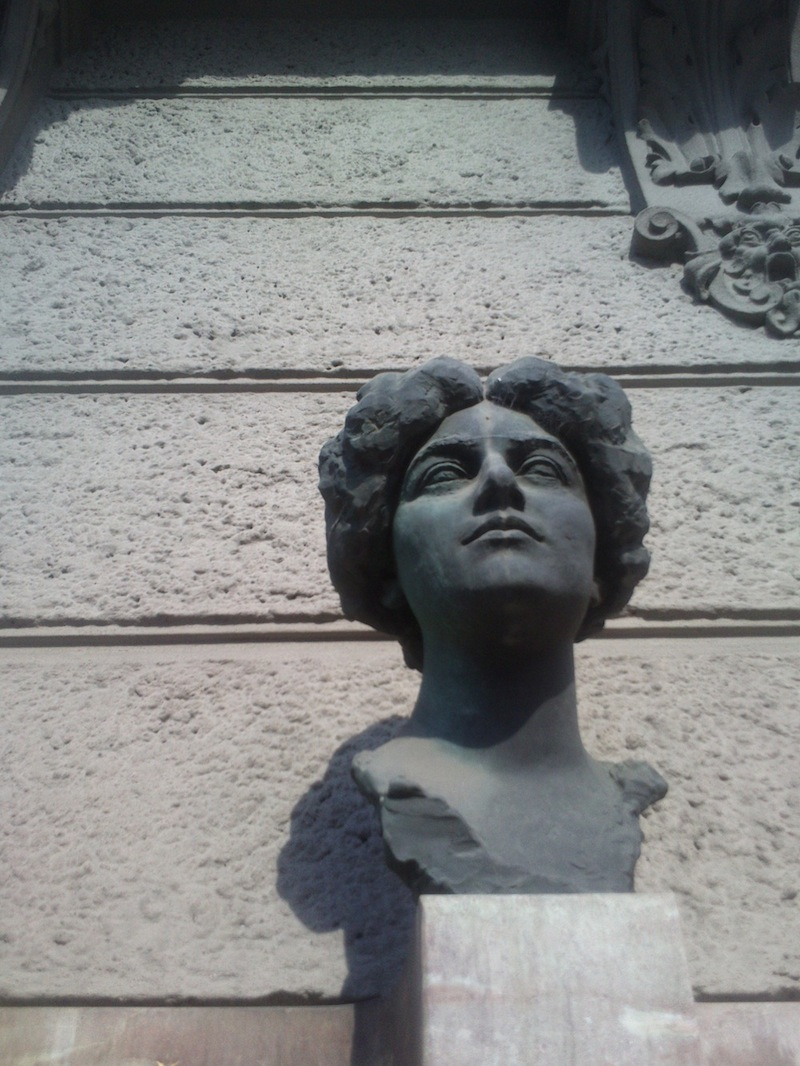
\includegraphics[width=6.0cm]{img/ema_a.png}
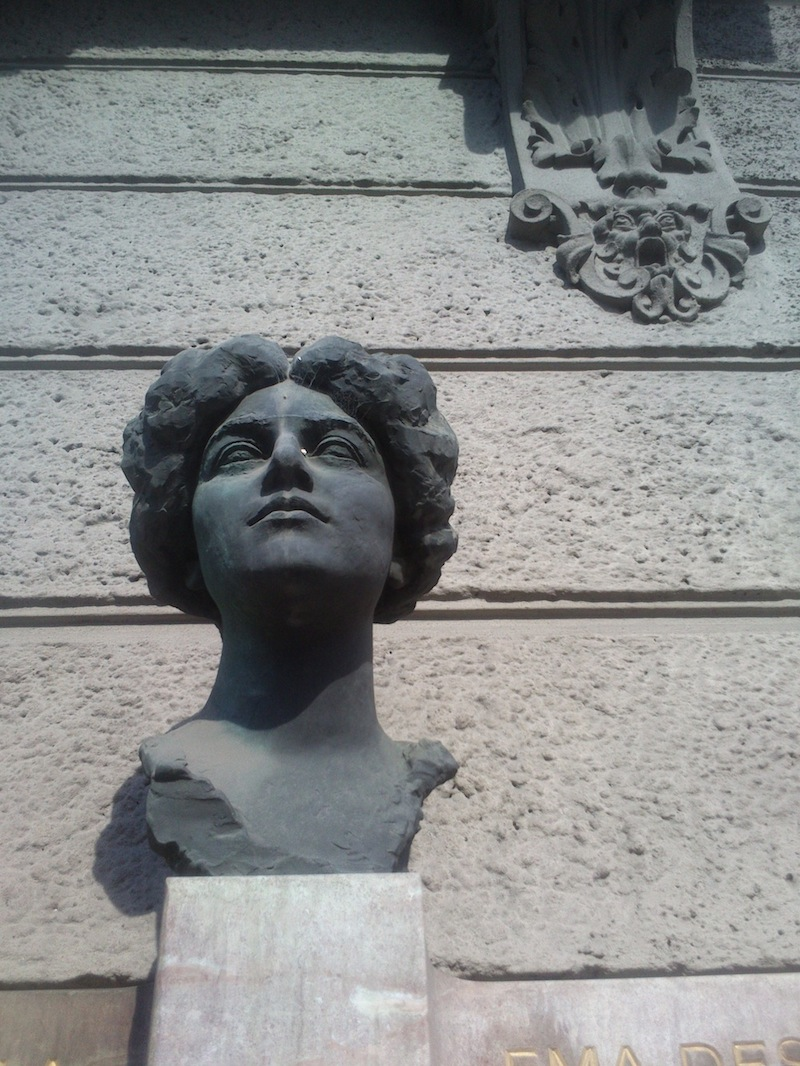
\includegraphics[width=6.0cm]{img/ema_b.png}}

\centerline{
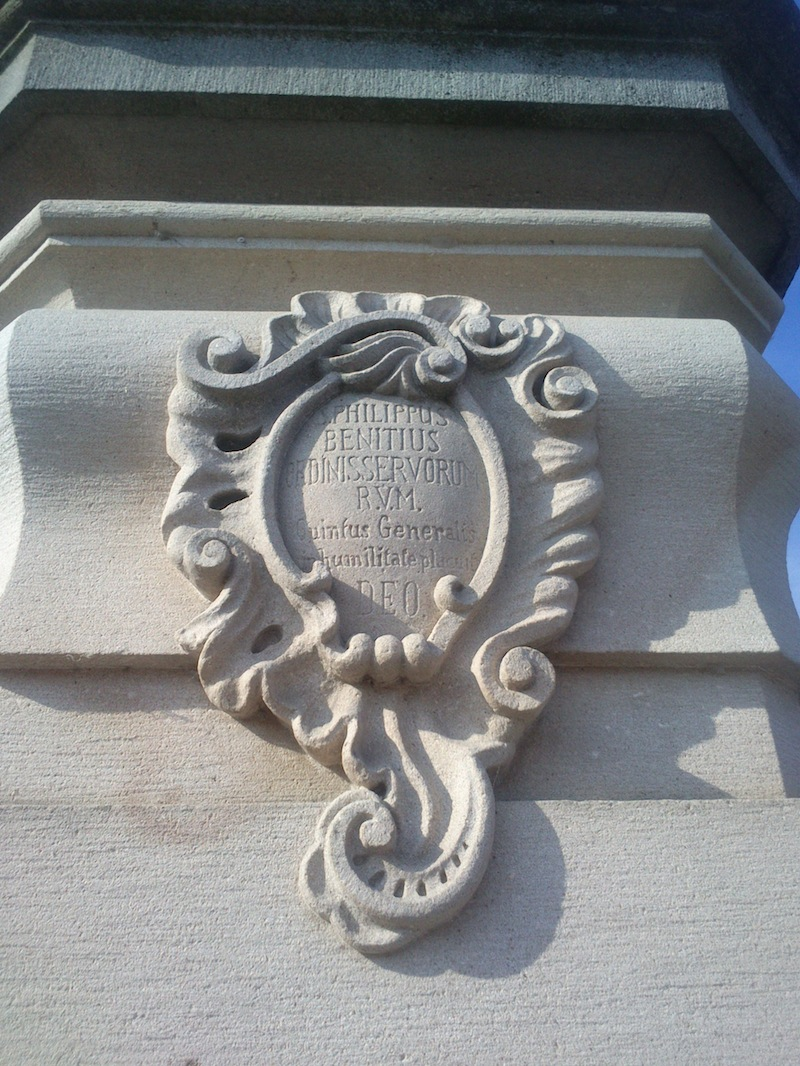
\includegraphics[width=6.0cm]{img/memorial_a.png}
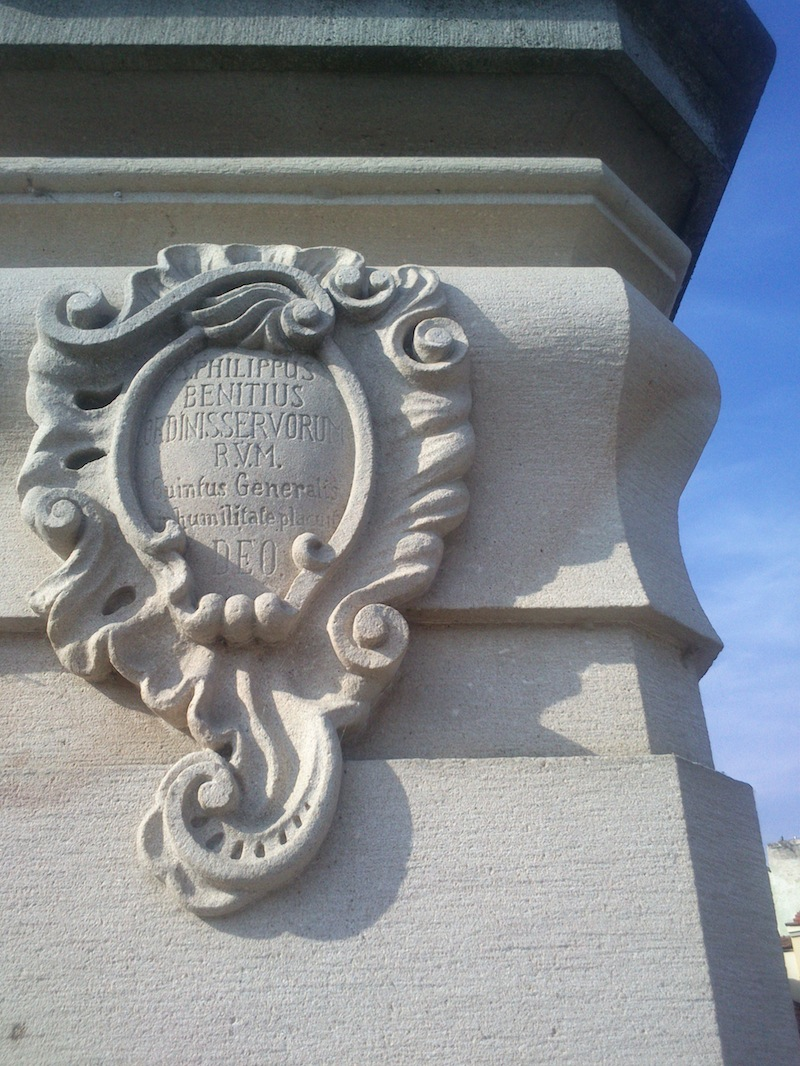
\includegraphics[width=6.0cm]{img/memorial_b.png}}

\caption{An example of input data.}
\label{fig:input_samples}
\end{figure}





\section{Results}
For the input data shown in Figure \ref{fig:input_samples} the results seem satisfying.
For this kind of input the SURF detector works properly.
It detects sufficient amount of keypoints and after filtering there remain enough good matches to get the information about the depth of some parts of the input images.

\begin{figure}[h]
\centerline{
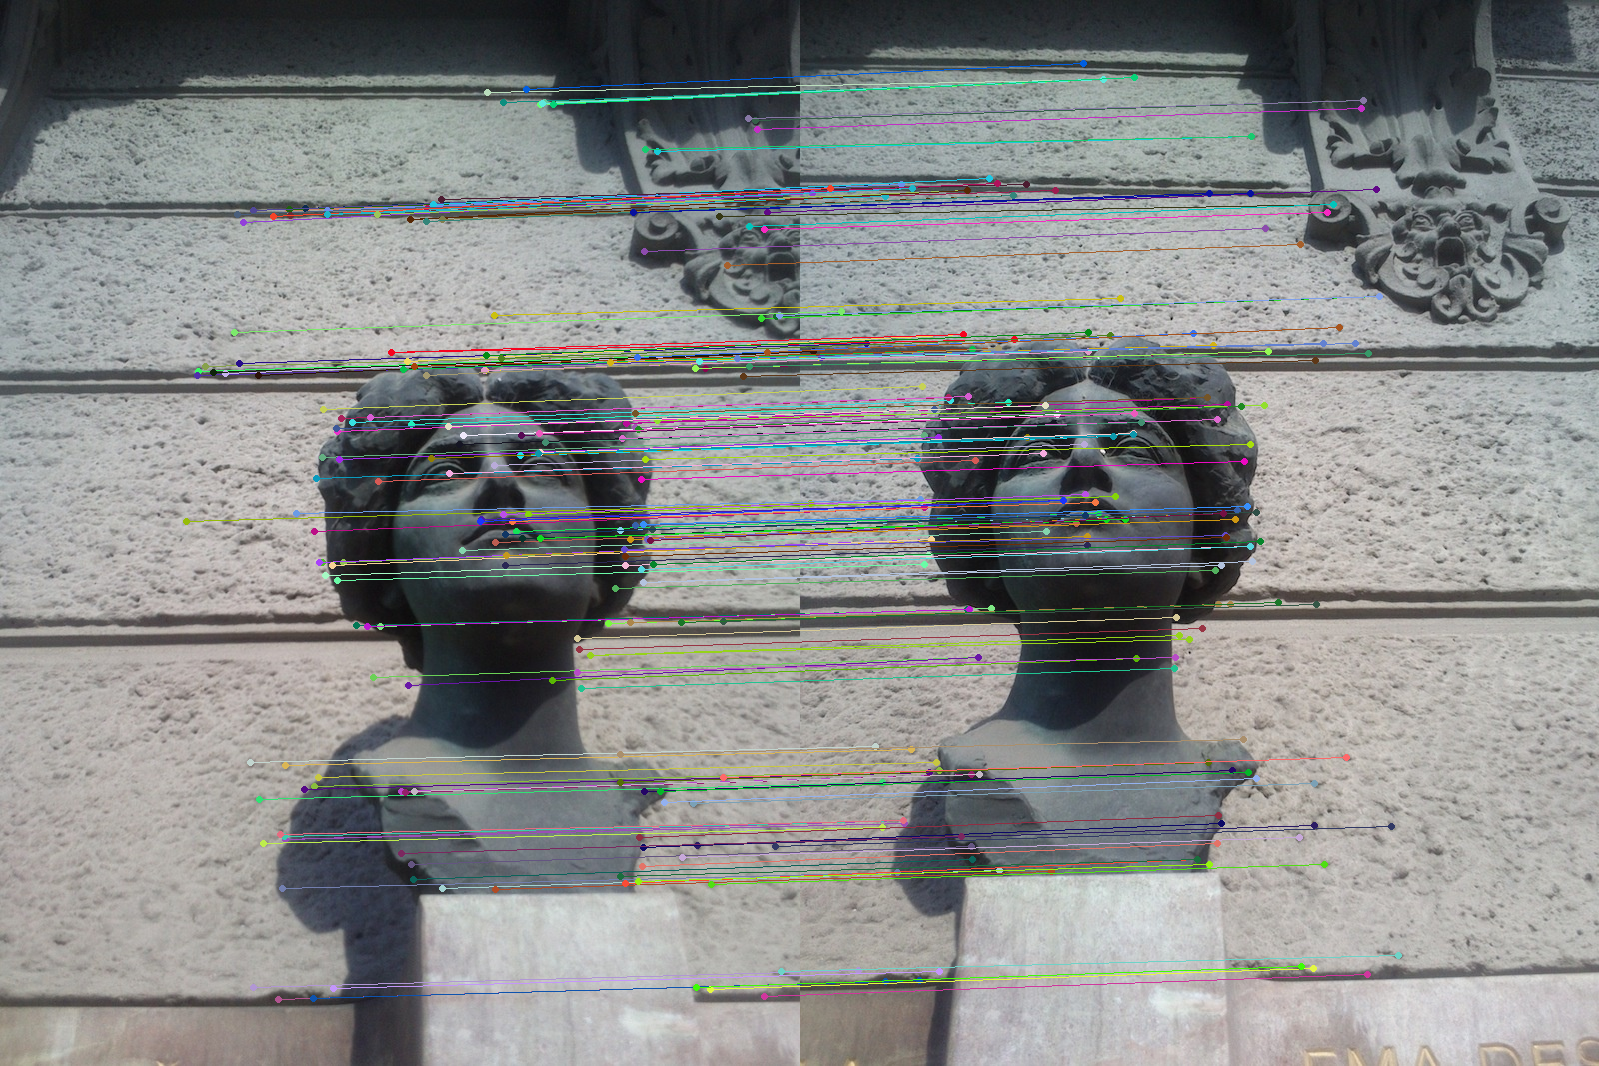
\includegraphics[width=12.0cm]{img/ema_matching.png}}
\centerline{
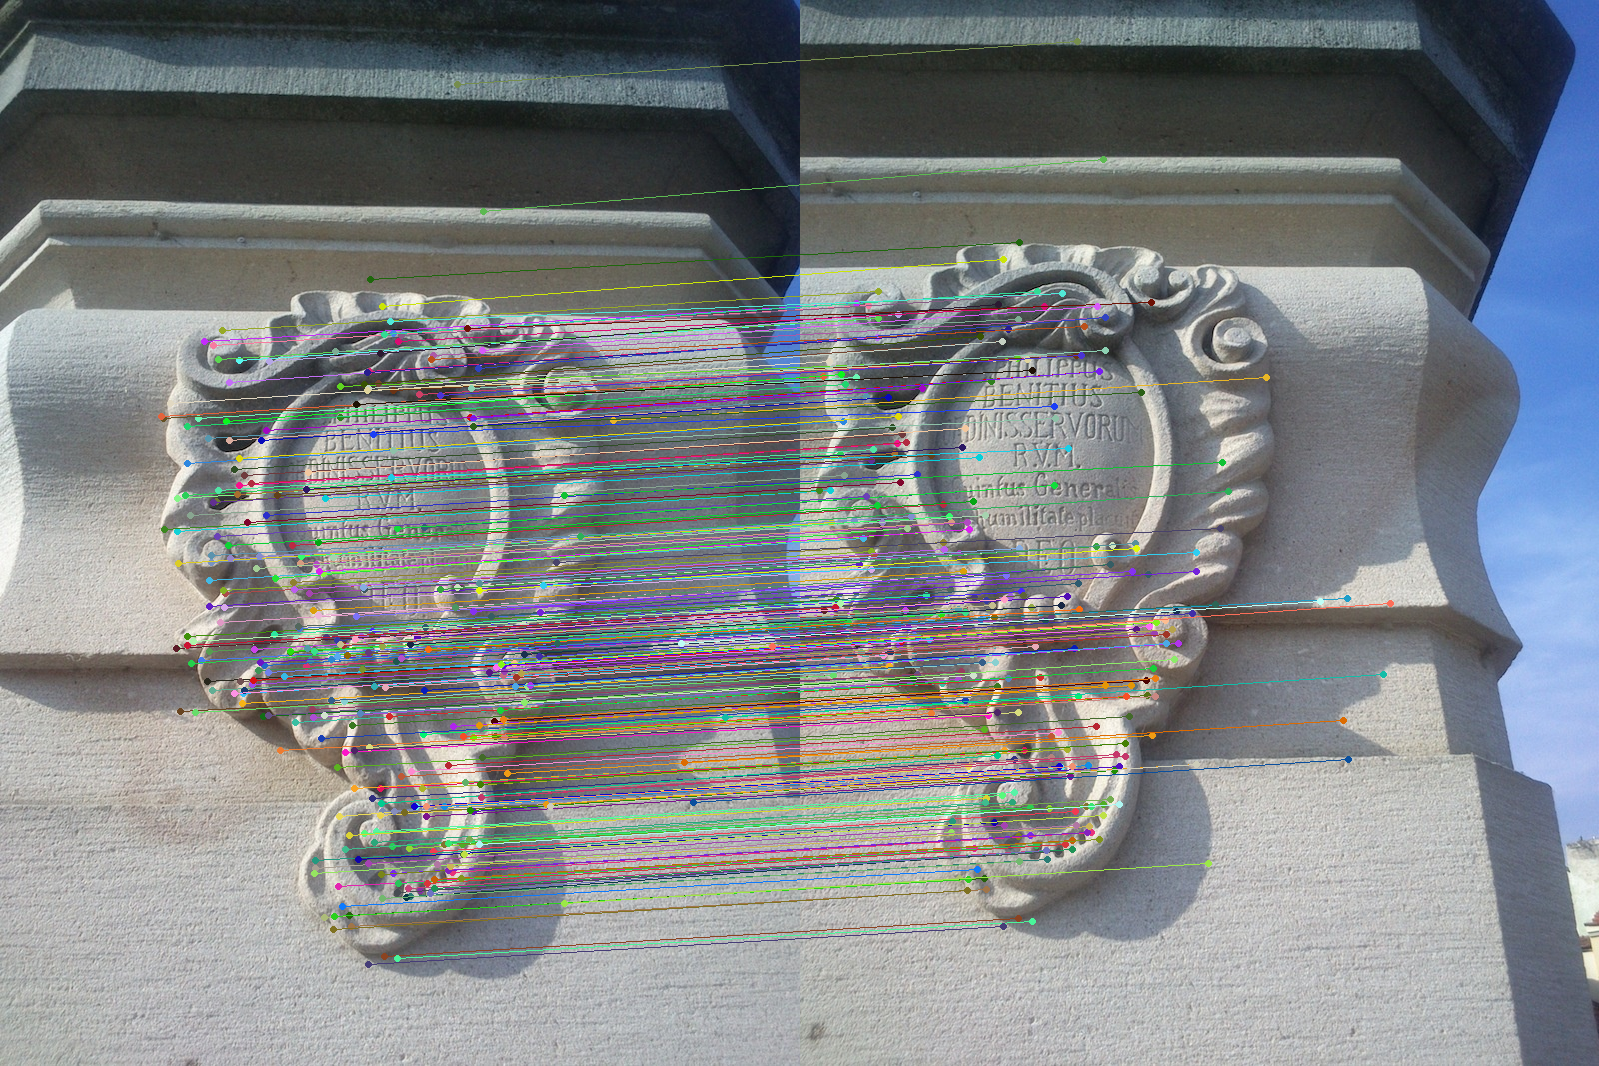
\includegraphics[width=12.0cm]{img/memorial_matching.png}}
\caption{The result of SURF matching.}
\label{fig:matching}
\end{figure}

For the pair of the images of a bust of Ema Destinová we get a 3D model shaping the head and a part of a wall in the background.
The second mentioned pair of input images gives us a result as an inclined plane in the angle of the memorial in the picture.
These results are comparable with the real appearance of the scenes.

\begin{figure}[h]
\centerline{
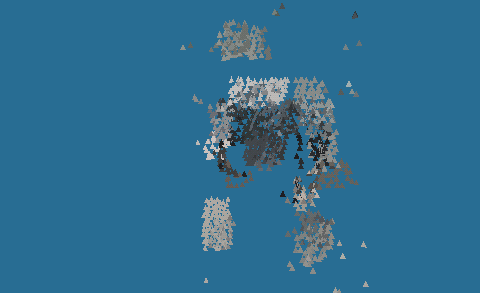
\includegraphics[width=7.0cm]{img/ema_3Dresult.png}

\includegraphics[width=7.0cm]{img/memorial_3Dresult.png}}
\caption{The output as a 3D model of disparity. The model of Ema Destinová sculpture (left) and of a memorial (right).}
\label{fig:outupt_samples}
\end{figure}

On the other hand for images with noise or images which are not highly textured, the result is usually a bunch of mismatches so the 3D model does not correspond to the reality.

\begin{figure}[h]
\centerline{

\includegraphics[width=7.0cm]{img/bad_input1.png}

\includegraphics[width=7.0cm]{img/bad_input2.png}}
\centerline{
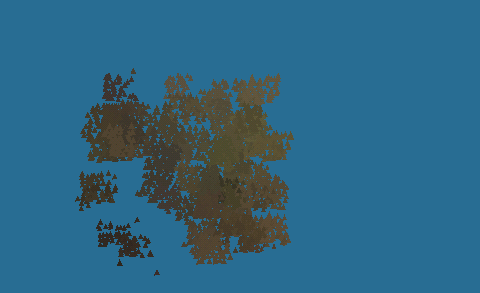
\includegraphics[width=7.0cm]{img/bad_result.png}}

\caption{An example of an input and output of a scene that does not give a good result.}
\label{fig:bad_example}
\end{figure}


